% Generated by paper/scripts/generate_tables.py; do not edit by hand.
\begin{figure}[!htbp]
\centering
\resizebox{0.92\linewidth}{!}{%
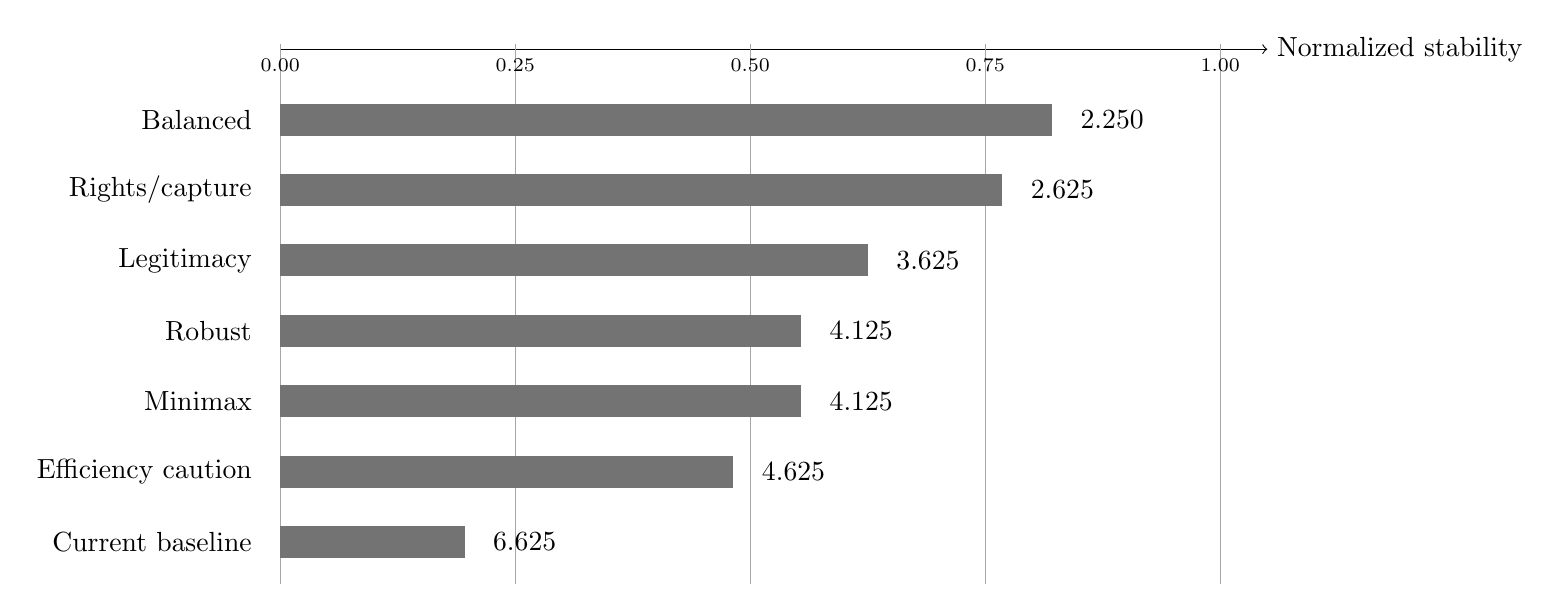
\begin{tikzpicture}[x=4.7in,y=0.80in]
\draw[->] (0,0) -- (1.05,0) node[anchor=west] {Normalized stability};
\foreach \x/\lab in {0/0.00,0.25/0.25,0.50/0.50,0.75/0.75,1.00/1.00} {
  \draw[black!35] (\x,0.03) -- (\x,-3.34);
  \node[anchor=north] at (\x,0) {\scriptsize \lab};
}
\node[anchor=east] at (-0.02,-0.44) {Balanced};
\fill[black!55] (0,-0.54) rectangle (0.821,-0.34);
\node[anchor=west] at (0.841,-0.44) {2.250};
\node[anchor=east] at (-0.02,-0.88) {Rights/capture};
\fill[black!55] (0,-0.98) rectangle (0.768,-0.78);
\node[anchor=west] at (0.788,-0.88) {2.625};
\node[anchor=east] at (-0.02,-1.32) {Legitimacy};
\fill[black!55] (0,-1.42) rectangle (0.625,-1.22);
\node[anchor=west] at (0.645,-1.32) {3.625};
\node[anchor=east] at (-0.02,-1.76) {Robust};
\fill[black!55] (0,-1.86) rectangle (0.554,-1.66);
\node[anchor=west] at (0.574,-1.76) {4.125};
\node[anchor=east] at (-0.02,-2.20) {Minimax};
\fill[black!55] (0,-2.30) rectangle (0.554,-2.10);
\node[anchor=west] at (0.574,-2.20) {4.125};
\node[anchor=east] at (-0.02,-2.64) {Efficiency caution};
\fill[black!55] (0,-2.74) rectangle (0.482,-2.54);
\node[anchor=west] at (0.502,-2.64) {4.625};
\node[anchor=east] at (-0.02,-3.08) {Current baseline};
\fill[black!55] (0,-3.18) rectangle (0.196,-2.98);
\node[anchor=west] at (0.216,-3.08) {6.625};
\end{tikzpicture}
}
\caption{Average-rank stress stability across the focused bridge cases. Bar labels show average stress rank; lower rank is better.}
\end{figure}
